\chapter{Literature Review}

\section{History of Nuclear Fuel Cycle Simulators}
% What is a nuclear fuel cycle
The \gls{NFC} represents the life cycle of nuclear fuel from initial
extraction, processing, use in reactors, and eventually to 
final disposal.
It is a complex system of facilities and mass flows 
that are combined to meet the goal of providing nuclear energy 
in the 
form of electricity \cite{yacout_modeling_2005}.
An open \gls{NFC} is if used fuel is not reprocessed and a 
closed \gls{NFC} is if used fuel is reprocessed. 
Presently, the \gls{US} has an open \gls{NFC}. 
Whereas, an example of a country that has a 
closed \gls{NFC} is France. 

% Purpose of NFCSims 
\glspl{NFCSim} are system analysis tools used to evaluate 
quantitative measures of performance related to the dynamics of 
a \gls{NFC} on both high and low resolution. 
An example of a high-resolution element is the plutonium 
concentration in a single used fuel bundle, and an example 
of a low-resolution element is total electricity produced. 
The purpose of \glspl{NFCSim} is to better understand the 
dependence between various input parameters and components 
in the \gls{NFC} system and the impact of their variations on 
the system's performance. 
The results of \glspl{NFCSim} are being used to guide research 
efforts, advise future design choices and to provide 
decision makers with a transparent tool for evaluating \glspl{FCO} 
to inform big-picture policy decisions \cite{yacout_modeling_2005}.

% Where are NFC codes from 
Historically, international national laboratories have driven 
development and are the major users of \gls{NFCSim} tools. 
However, due to propriety access to these tools, universities and 
other non-laboratory organizations have taken to creating their 
own tools. 
Table \ref{tab:nfctools} shows a breakdown of the \glspl{NFCSim}
and the organization(s) associated with it. 

\begin{table}[]
    \centering
    \resizebox{0.7\textwidth}{!}{%
    \begin{tabular}{|l|l|}
    \hline
    \textbf{\gls{NFCSim}} & \textbf{Organization(s) associated with it}                                    \\ \hline
    \Cyclus \cite{huff_fundamental_2016}                & \begin{tabular}[c]{@{}l@{}}\gls{UW} \\ \gls{UIUC}\end{tabular} \\ \hline
    DYMOND \cite{yacout_modeling_2005},                                & \gls{ANL}                                                                                               \\ \hline
    ORION  \cite{gregg_analysis_2012}                                & \gls{NNL}                                                                                             \\ \hline
    VISION \cite{jacobson_vision:_2006}                                & \gls{INL}                                                                                               \\ \hline
    COSI   \cite{coquelet-pascal_cosi6:_2015}                                &   \gls{CEA}                    \\ \hline
    CLASS  \cite{mouginot_class_2012}                                &  \begin{tabular}[c]{@{}l@{}}\gls{CNRS} \\ \gls{IRSN}\end{tabular}                                      \\ \hline
    DESAE  & \gls{OECD} \\ \hline
    \end{tabular}%
    }
    \caption{Nuclear Fuel Cycle Simulator Tools and their corresponding organizations.}
    \label{tab:nfctools}
    \end{table}

% what is agent, what is fleet
One of the major distinctions between the various \glspl{NFCSim}
is fleet-level or agent-level modeling of facilities and materials. 
Fleet-based models do not distinguish between discrete facilities 
or materials, but instead lump them together into fleets and streams. 
The advantages of this method is a simpler code structure and 
lower computational cost. 
Agent-based models treats facilities and materials as discrete 
objects. 
The advantages of this method are more flexible simulation control
and ease of simulating a wide range of scenarios with new 
technologies.  

% why is it good that there are multiple tools 
% benchmark against each other
Efforts have been made towards benchmarking \gls{NFCSim} 
tools against each other to verify them 
\cite{feng_standardized_2016,guerin_benchmark_2009}. 
These comparison studies assist developers in modifying the
codes to more realistically model the \gls{NFC}. 
Also, by upholding the \gls{NFCSim} tools to high level agreement, 
stakeholders and decision makers can have more confidence in 
prediction results generated by \gls{NFCSim} tools and trust them 
to inform on potential strategic and policy decisions
\cite{feng_standardized_2016}. 

\section{Transition Scenarios}
In Chapter \ref{chap:1}, the history and motivation of
\gls{NFC} transition scenario research was described.
More detail about transition scenario studies will be given 
in this section. 

The evaluation and screening study identified 40 promising 
\glspl{EG} to represent a comprehensive set of 
\gls{FCO} \cite{wigeland_nuclear_2014}. 
To access the performance of each \gls{EG}, the study
used 9 evaluation criteria: nuclear waste management, 
proliferation risk, nuclear material security risk, 
safety, environmental impact, resource utilization, 
development and deployment risk, institutional issues, and 
financial risk.  
The conclusion of the study is that fuel cycles
involving continuous recycling of co-extracted U/Pu or U/TRU in 
fast spectrum critical reactors consistently scored high overall 
performance.
In the study, these fuel cycles were referred to as EG23, EG24, 
EG29 and EG30. 
Table \ref{tab:eg} provides a description of the current 
\gls{US} \gls{EG} and the promising \glspl{EG}. 
These \glspl{EG} were evaluated at an equilibrium state to 
understand the end-state benefits of each evaluation group (EG).
Knowing the most promising end state \glspl{EG}, 
the next step is to evaluate and compare the transition process 
from the current EG01 
state to these promising \glspl{EG} \cite{feng_standardized_2016}. 
\begin{table}[]
    \centering
    \caption{Descriptions of the current and other high performing nuclear fuel cycle evaluation groups described in the evaluation and screening study \cite{wigeland_nuclear_2014}.}
    \label{tab:eg}
        \footnotesize
        \begin{tabularx}{\textwidth}{l|LLL}
            \hline
        \textbf{Fuel Cycle}                                               & \textbf{Open or Closed} & \textbf{Fuel Type}                                                              & \textbf{Reactor Type}                                                                           \\ \hline
        \textbf{\begin{tabular}[c]{@{}l@{}}EG01\\ (current)\end{tabular}} & Open                                                               & Enriched-U                                                                      & Thermal critical reactors                                                                       \\ 
        \textbf{EG23}                                                     & Closed                                                             & \begin{tabular}[c]{@{}l@{}}Recycle of U/Pu \\ with natural-U fuel\end{tabular}  & Fast critical reactors                                                                          \\ 
        \textbf{EG24}                                                     & Closed                                                             & \begin{tabular}[c]{@{}l@{}}Recycle of U/TRU \\ with natural-U fuel\end{tabular} & Fast critical reactors                                                                          \\ 
        \textbf{EG29}                                                     & Closed                                                             & \begin{tabular}[c]{@{}l@{}}Recycle of U/Pu \\ with natural-U fuel\end{tabular}  & \begin{tabular}[c]{@{}l@{}}Fast critical reactors and \\ thermal critical reactors\end{tabular} \\ 
        \textbf{EG30} & Closed                                                             & \begin{tabular}[c]{@{}l@{}}Recycle of U/TRU \\ with natural-U fuel\end{tabular} & \begin{tabular}[c]{@{}l@{}}Fast critical reactors and \\ thermal critical reactors\end{tabular} \\ \hline
    \end{tabularx}
\end{table}


\section{\glspl{NFCSim} Transition Scenario Capabilities}
% what has been done for transition scenarios so far
Both \gls{NFCSim} tools used in this thesis, \Cyclus and DYMOND,
were verified by a benchmarking effort for use of 
\gls{NFCSim} tools to conduct transition scenario analyses
\cite{feng_standardized_2016,bae_standardized_2019}.
The reference problem used in the benchmark was a simplified 
transition of one hundred 1000-MWe \glspl{LWR} to a fleet 
of 333.3-MWe \gls{SFR} fleet. 
They were found to have excellent agreement with the 
spreadsheet solution and other \gls{NFC} codes.  
This benchmarking effort proved that these \glspl{NFCSim}
are capable of simulating a simple transition scenario. 
However, it acknowledged that there needs to be more efforts 
to model realistic transition scenarios to evaluate the
flexibility of the \glspl{NFCSim} \cite{feng_standardized_2016}.
In-depth descriptions about \Cyclus and DYMOND is provided in 
chapter \ref{chap:3}.

% brown paper 
% teddy thesis for cyclus capabilties 

\section{\glspl{NFCSim} Sensitivity Analysis}
% SA for NFCs vs SA for NFC transition scenarios 

To enable \glspl{NFCSim} to produce insightful and 
flexible results to inform policy decisions, it is necessary 
to be able to quantify and include all the 
subtleties of each segment of the \gls{NFC} through system analysis 
and sensitivity studies \cite{passerini_systematic_2014}. 
A transition scenario is simulated to predict the future, 
however when implemented in the real world, it will deviate from 
the optimal scenario. 
Therefore, sensitivity analysis studies is necessary to determine 
how variation in different parameters will impact the 
progression and final state     of the transition scenario. 

Previous work towards \gls{SA} and \gls{UQ} of \gls{NFC} 
simulations used these terms interchangeably. 
This is because \gls{UQ} in \glspl{NFCSim} are seen as design 
uncertainties. 
For example, a pyrochemical reprocessing facility has never been 
built, therefore, its throughput is viewed as a design parameter 
that can be varied. 
By conducting \gls{SA}/\gls{UQ} on the throughput design 
parameter, the impact on important output parameters can be 
determined. 
By conducting similar studies on a large set of input parameters, 
it will indicate which parameters have large impacts, giving a clear 
picture of where a closer sensitivity study should be conducted and 
where additional modeling detail should be added. 
It will also identify which parameters the system is relatively 
insensitive to \cite{noauthor_effects_2017}. 

\gls{SA} is a technique used to determine how 
varying input variable(s) will impact
output variables for a given scenario. 
Many assumptions are made when setting up the simulation scenarios, 
therefore, \gls{SA} will assist in the evaluation of
sensitivity of the output of the scenario to each of these 
assumptions.  
There are three types of sensitivity analysis: one-at-a-time (OAT), 
synergistic and global. 

\subsection{One-at-a-time Sensitivity Analysis}
OAT is basic \gls{SA} that focuses on estimating the lone effect 
of one input variable. 
This approach gives the local impact of each variable on the 
output parameters of interest. 
OECD conducted a OAT sensitivity analysis \cite{noauthor_effects_2017} 
on key \gls{NFC} input parameters
and quantified the impacts on the selected output parameters. 
The base scenario used has a duration of 200 years, begins 
with a fleet of \glspl{PWR} and transitions to \glspl{SFR} while 
maintaining constant electricity production. 
They varied each parameter independently for three cases: 
the base case, a high case, and a low case. 
The results of these variations on the output parameters 
are expressed in tornado plots and sensitivity tables. 
Figure \ref{fig:oecd-sensitivitytable} shows the sensitivity table
provided by the benchmark that gives an overview of their analysis. 
Figure \ref{fig:oecd-tornado} shows an example tornado plot that represents 
the sensitivity of separated Pu in storage to the various input parameters. 

\begin{figure}[]
	\begin{center}
		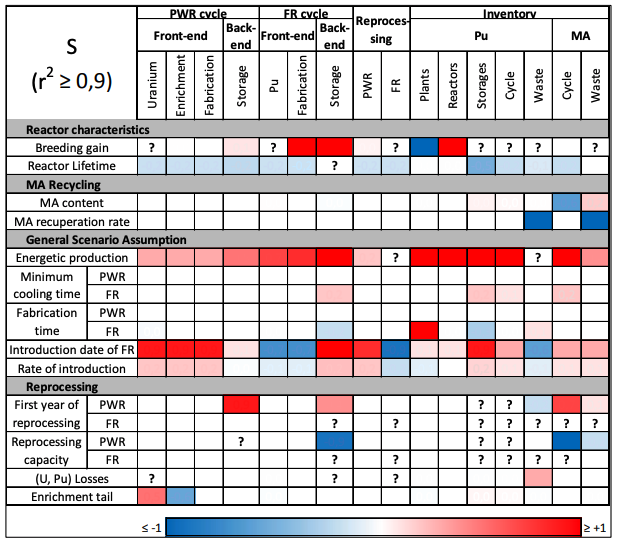
\includegraphics[scale=0.55]{./figures/oecd-sensitivitytable.png}
	\end{center}	
		\caption{Sensitivity Table that provides an overview of the sensitivity 
		of each output parameter to the respective input parameters \cite{noauthor_effects_2017}.}
	\label{fig:oecd-sensitivitytable}
\end{figure}

\begin{figure}[]
	\begin{center}
		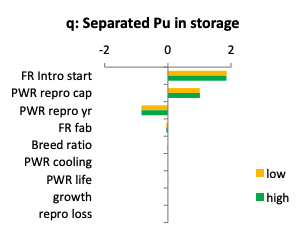
\includegraphics[scale=0.65]{./figures/oecd-tornado.png}
	\end{center}	
		\caption{Tornado plot showing the sensitivity of separated Pu in 
		storage to each input parameter \cite{noauthor_effects_2017}.}
	\label{fig:oecd-tornado}
\end{figure}

\subsection{Synergistic Sensitivity Analysis}
Synergistic \gls{SA} involves multidimensional parametric 
input sweeps to view the impact of synergistic changes of input 
variables on specific output variables. 
It is possible to conduct synergistic \gls{SA} by varying 
two input variables simultaneously and viewing their 
combined impact on each output parameter or a combination 
of weighted output parameters. 
Figure \ref{fig:passerini_payoff} shows an example of this analysis.
Thermal reprocessing and fast reactor technology introduction dates
were varied and an objective payoff surface representing a combination 
of multiple optimization criteria is shown. 
This method of synergistic study informs on the local effects of 
two input variables on the system, however, it fails to inform 
on the global sensitivity of the system. 

\begin{figure}[]
	\begin{center}
		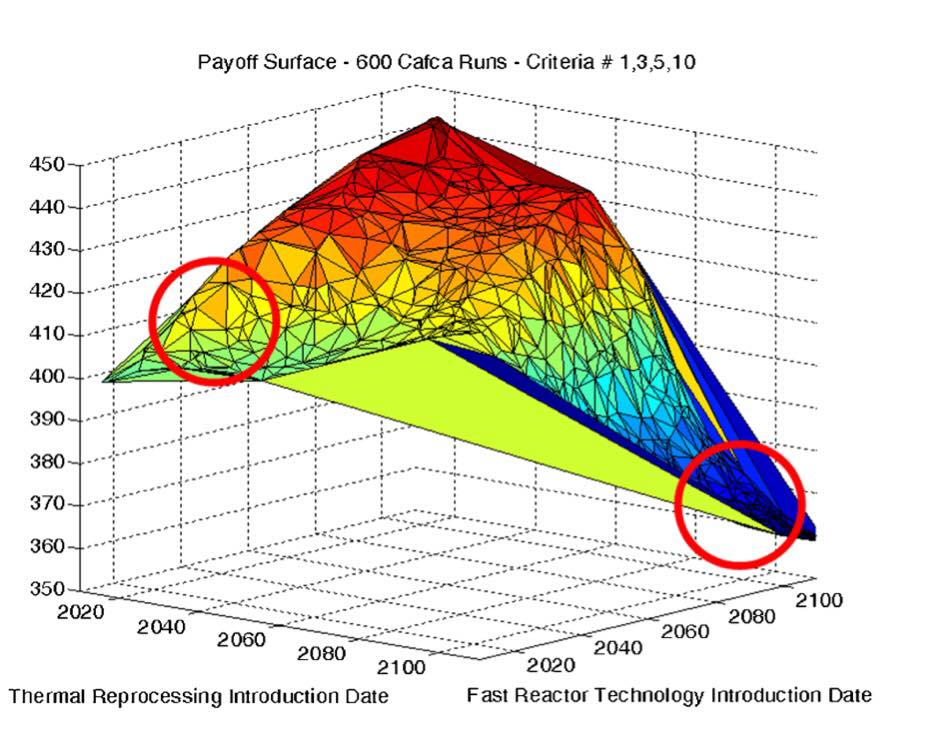
\includegraphics[scale=0.25]{./figures/passerini_payoff.jpg}
	\end{center}	
		\caption{Optimization Surface of the payoff when varying thermal 
		reprocessing and fast reactor technology introduction date
		\cite{passerini_systematic_2014}}
	\label{fig:passerini_payoff}
\end{figure} 

\subsection{Global Sensitivity Analysis}
To fully consider the synergistic effects of
simultaneous variation of the input variables, a variance 
based approach can be used instead \cite{thiolliere_methodology_2018}.
Thiolliere et al conducted a global sensitivity analysis of a 
\gls{NFC} scenario by using Latin Hypercube sampling 
to generate Sobol' indices. 
The scenario was a simulation of a simplified PWR-UOX MOX fuel 
fleet. 
Sobol Indices' provide the global sensitivity effect of each input 
variable by decomposing the variance of the output into fractions 
that are attributed to inputs or sets of inputs. 
Essentially it tells us which design parameter have the most 
influence on the response quantities. 
Large Sobol' indices' signifies that variation in that 
input variable is more impactful to the output parameter. 

\subsection{Main Takeaways}
\gls{SA} studies of \glspl{NFC} have previously been used to narrow 
down and compare a wide range of \gls{NFC} scenarios to determine 
the ideal scenario end types. 
The conclusions are that the main trade-off for fuel cycle 
optimization is economics 
versus other metrics such as environmental impact, proliferation 
risk \cite{passerini_systematic_2014}.
It was determined that the desired fuel cycle end states 
were EG23, EG24, EG29,s and EG30.
These \gls{SA} studies focused on high level input 
parameters such as reactor and reprocessing technologies etc.
However, limited sensitivity studies have been performed to 
evaluate specific transition scenarios that describe the transition 
from the current to desired end states.
The only relevant sensitivity study was conducted by OECD 
\cite{noauthor_effects_2017}, however it was a basic OAT 
\gls{SA}.   
Therefore, synergistic \gls{SA} studies focused on
lower level input parameters such as cooling time, 
date of introduction of reprocessing/reactor 
technologies, ratio of technology types should be conducted to 
understand the nuances of the variation of these low-level parameters. 
Through synergistic \gls{SA}, these transition scenarios can be 
further optimized and used to inform other nuclear research areas 
such as reprocessing facility design etc. 
